% ============================================================
% IEEE Transactions (Q1) format - IEEEtran class, two columns.
% Compiles on Overleaf or texlive-full (IEEEtran is standard).
% ============================================================
\documentclass[10pt,journal]{IEEEtran}

\usepackage[utf8]{inputenc}
\usepackage[T1]{fontenc}
\usepackage{lmodern}
\usepackage{amsmath,amssymb}
\usepackage{booktabs}
\usepackage{graphicx}
\usepackage{cite}
\usepackage[hidelinks]{hyperref}

\begin{document}

\title{Structured Sparsity in Transformer Feed-Forward Layers:\\
A Controlled Study of the Coverage--Depth--Communication Trade-off}

\author{Mustafa Selman Durmaz%
\thanks{The author was supported by the TUBITAK ULAKBIM TRUBA/ARF Training Program
(project code \texttt{egitimg35}). E-mail: dselman1134@gmail.com.}%
\thanks{The numerical calculations reported in this paper were fully performed at TUBITAK
ULAKBIM, High Performance and Grid Computing Center (TRUBA resources).}}

\markboth{TUBITAK ULAKBIM TRUBA/ARF Training Program, August 2026}%
{Durmaz: Structured Sparsity in Transformer FFN Layers}

\maketitle

\begin{abstract}
In large language models, feed-forward network (FFN) layers hold a large fraction of the
parameters and compute and consist of two dense rectangular weight matrices. We ask whether
the \emph{density} of these matrices is a necessity or a relaxable assumption, and study seven
connectivity patterns (dense, ring, small-world, random, block-diagonal, mosaic, butterfly)
under an \emph{equal-parameter and equal-FLOP} constraint. Experiments are run on eight NVIDIA
H200 accelerators at three scales (layer, architecture, distributed); we report 326 training
runs with multiple random seeds and significance tests. We obtain four main findings. First,
at a fixed density, model quality is determined not by the \emph{name} of the pattern --- but
per-layer \emph{coverage} does not suffice either: two patterns with identical coverage can
differ by $9.6\sigma$. We instead define the \emph{mixing depth} $\tau$ (the number of layers
required for every output to reach every input); patterns with equal $\tau$ are statistically
indistinguishable ($\sigma\le0.95$), and the boundary between $\tau\le L$ and $\tau>L$ is
significant at every density. We test $\tau$ with two pre-registered, falsifiable predictions:
freezing the butterfly's stage should drop its quality onto that of block-diagonal (measured
to within $0.14\sigma$), and in the sparsest regime butterfly --- the only pattern that
completes its mixing --- should overtake ring despite having half its coverage (it does, by
$2.5\sigma$). Second, the effect of depth is not monotone: the gap closes at the $\tau$
threshold and reopens beyond it through saturation. Third, the butterfly's apparent advantage
over ring largely dissolves under self-guided training ($12.0\sigma \to 1.5\sigma$), showing
that much of what looks architectural is optimization difficulty. Fourth, in the distributed
setting butterfly sharding reduces the number of communication peers
per layer from $P{-}1$ to $1$, but this gain comes with a small quality cost that shrinks with
scale. We show that this trade-off rests on an information-theoretic bound (full per-layer
coverage and single-peer communication cannot coexist in one layer) and quantify, via a
decision model, the infrastructure conditions under which the method is rational. The
contribution is not a new method but a controlled map of the communication--quality trade-off
in distributed FFN design.
\end{abstract}

\begin{IEEEkeywords}
Structured sparsity, feed-forward network, distributed training, tensor parallelism, butterfly
matrices, communication efficiency, large language models.
\end{IEEEkeywords}

\IEEEpeerreviewmaketitle

% ============================================================
\section{Introduction}
% ============================================================
\IEEEPARstart{I}{n} Transformer-based \cite{vaswani2017} large language models, the growth of
parameter scale is the primary driver of performance \cite{kaplan2020,chinchilla2022} but also
creates an infrastructure bottleneck due to memory
bandwidth and inter-accelerator communication limits. About two thirds of a Transformer
layer's parameters lie in the feed-forward network (FFN), which consists of two \emph{dense}
matrices that widen the hidden dimension to four times the model dimension
($d \rightarrow 4d$) and narrow it again ($4d \rightarrow d$). To reduce parameter and compute
cost, replacing these matrices with low-rank, block-diagonal, butterfly, or general sparse
forms has become a broad research area.

This literature has advanced along two separate axes. The first focuses on \emph{single-device
efficiency}: structured matrices reduce parameters and theoretical operation count, but their
effect on quality and real speed depends on the implementation. The second focuses on
\emph{distributed communication}: when a model does not fit on a single accelerator, techniques
such as Tensor Parallelism (TP) become mandatory and require an inter-device \emph{all-reduce}
collective at every layer. These two axes have mostly been studied independently.

We unite the two axes in a single controlled framework and ask: how does abandoning the dense
FFN matrix assumption affect quality, speed, and distributed communication load, when
parameters and operation count are held fixed? The crucial aspect is the ``equal-parameter and
equal-FLOP'' constraint: a comparison that reduces parameter count leaves it ambiguous whether
the difference comes from the sparse model being \emph{smaller} or from its \emph{shape}. We
widen the hidden layer and lower the density so that all variants have the same parameter and
operation count; the only variable that changes is the \emph{shape} of the weight matrix.

\emph{Motivation.} The initial motivation was the scenario of uniting geographically scattered
compute resources for a single model training run. In that scenario the bottleneck is not total
compute but the narrow link between nodes. If an FFN's weight matrix has a local connectivity
structure, then when it is sharded each shard may only need to communicate with a few
neighbors; this offers the hope of operating over narrow links, unlike dense TP where every
node communicates at every layer. This work directly and quantitatively tests that hope.

\emph{Nature of the work.} This is not a method-proposal paper but a controlled empirical
characterization. Our aim is not to declare a new architecture superior; it is to measure,
with control groups and statistical significance, which design choice gains or loses what under
which conditions. A significant portion of our results is negative or nuanced, and we consider
the honest reporting of such results a core value of the study.

Our contributions are: (1) We compare seven FFN topologies under the equal-parameter/FLOP
constraint, show that per-layer coverage fails to explain quality, and propose the
\emph{mixing depth} $\tau$ in its place, testing it with pre-registered falsifiable
predictions. (2) We measure that the effect of depth reverses direction at the $\tau$
threshold --- incomplete mixing below it, saturation above it --- and, with a fixed-mask
control, disentangle the ``unstructured random is best'' finding from this second mechanism.
(3) On eight H200s, at equal per-rank parameters, we measure that butterfly
sharding reduces peers per layer from $P{-}1$ to $1$ and FFN communication by $\sim\!7\times$,
but that the end-to-end gain is limited to $\sim\!2\times$ due to the attention all-reduce.
(4) We state an information-theoretic bound under which full per-layer coverage and single-peer
communication are incompatible. (5) We quantify, with a decision model, the range of conditions
under which the method is rational.

% ============================================================
\section{Related Work}
% ============================================================
\emph{The parallelism stack.} The forms of parallelism used to train large models are
complementary: data parallelism reduces the memory burden by sharding optimizer state
(ZeRO \cite{zero2020}, FSDP \cite{fsdp2023}), pipeline parallelism splits layers across
devices \cite{gpipe2019}, and tensor parallelism splits a single layer and therefore requires
an all-reduce at every layer \cite{megatron2019,narayanan2021}. This work concerns the last of
these: whether the communication load of FFN tensor parallelism can be reduced by changing the
\emph{shape} of the weight matrix. Work on activation memory and sequence parallelism
\cite{korthikanti2023} and approaches that shard the attention layer \cite{ringattn2023} are
orthogonal to this axis.

\emph{Forms of sparsity.} The weight-sparsity literature is long: magnitude pruning
\cite{han2015}, the lottery ticket hypothesis \cite{frankle2019}, methods that redistribute
connections during training \cite{rigl2020}, and one-shot pruning \cite{sparsegpt2023}. On the
hardware side, NVIDIA's 2:4 structured sparsity \cite{nm2021} shows how narrow a structure must
be before a pattern translates into speedup. Expander networks drawn from graph theory
\cite{expander2018} design sparse layers through connectivity, with a motivation close to our
coverage intuition. Butterfly factorizations were first used to learn fast transforms
\cite{dao2019} and later generalized to sparse training \cite{pixelbutterfly2022}.

\emph{Structured FFN matrices.} Wei \emph{et al.} \cite{wei2024} observed optimization
instabilities when training low-rank FFNs from scratch and proposed self-guided training, which
uses a temporary dense branch early in training. The Monarch matrices of Dao \emph{et al.}
\cite{dao2022} are a product of two block-diagonal matrices up to permutation and, by exploiting
batched matrix-multiply (bmm) kernels, achieve up to $2\times$ speedup over dense multiply.
These works focus on single-device efficiency.

\emph{Dynamic sparsity: mixtures of experts.} The field's adopted route to sparsifying the FFN
is the mixture-of-experts (MoE), in which a router dispatches each token to a few experts
\cite{shazeer2017,gshard2021,switch2022}. This is a different kind of sparsity from the one we study. In MoE the
sparsity is \emph{input-dependent and dynamic}; the weight matrices themselves stay dense and
what is sparse is expert selection. Its distributed cost differs as well: expert parallelism
requires an \emph{all-to-all} per layer, a collective more expensive on narrow links than the
fixed-peer exchange we examine. The subject of this work is \emph{static structural} sparsity:
the pattern is fixed before training, the peer set is constant, and there is no routing cost.
The two approaches are orthogonal rather than competing; MoE's quality/throughput balance is
independent of the communication--coverage trade-off we measure.

\emph{Reducing communication on the optimization side.} The motivating goal of uniting
scattered resources over a narrow link has also been attacked without altering weight
structure: the local-SGD family \cite{stich2019} and DiLoCo \cite{diloco2023} synchronize nodes
every few hundred steps rather than every step, cutting communication by two orders of
magnitude, while SWARM \cite{swarm2023} and Petals \cite{petals2023} target unreliable and
heterogeneous nodes. That
approach changes the synchronization \emph{schedule}, not the shape of the matrix. Our findings
do not conflict with this literature but complement it: we show that pursuing the same goal
along the weight-structure axis runs into an information-theoretic bound
(Section~\ref{sec:bound}), which explains why the solution is sought on the optimization axis.

\emph{Pattern diversity and depth.} ShuffleSparse \cite{shufflesparse2025} showed theoretically
that fixed axis-aligned sparsity patterns cannot gain depth-multiplicative expressivity, whereas
depth-varying full-rank mixers can. We confirm this theory with independent measurement.

\emph{Distributed communication.} Tensor parallelism requires two all-reduces per layer, and
this communication can constitute a significant fraction of inference time \cite{flashcomm2024}.
Approaches that reduce communication with block-diagonal structure (BD-LoRA \cite{bdlora2025},
DeTransformer \cite{detransformer2024}) rely on fixed patterns and are mostly designed for
inference. The axis we study is using a depth-varying pattern as a distributed sharding
topology; in our search we found no work that jointly addresses expressivity and peer count.
Approaches that reduce communication on the attention side (sequence parallelism, ring
attention) are orthogonal to this axis and composable with the FFN-side gain; the
$\sim\!2\times$ end-to-end ceiling we measure (Section~\ref{sec:limits}, item 1) arises
precisely from not combining them.

% ============================================================
\section{Method}
% ============================================================
\subsection{Equal-parameter and equal-FLOP protocol}
A standard FFN is a dense intermediate of hidden size $4d$:
$\mathrm{FFN}(x) = W_{\downarrow}\,\sigma(W_{\uparrow}x)$, with
$W_{\uparrow}\in\mathbb{R}^{4d\times d}$, $W_{\downarrow}\in\mathbb{R}^{d\times 4d}$ and total
parameters $8d^2$. To compare a sparse variant fairly, we widen the hidden size to $M\!\cdot\!d$,
lower the density to $4/M$, and keep the number of nonzeros (nnz) equal to the dense model:
\begin{equation}
h = M\,d, \qquad \text{density} = \frac{4}{M}, \qquad \mathrm{nnz} = 8d^2 .
\end{equation}
Thus $M=4$ is the dense model itself, $M=8$ is density $1/2$, $M=16$ is density $1/4$. Under this
protocol all variants have the same parameter and operation count; the only thing that changes is
the shape of the weight matrix.

\subsection{Connectivity patterns}
We compare seven FFN patterns (Table~\ref{tab:variant}). The \emph{random} pattern is a critical
control group: only it can separate whether a difference comes from structure or merely from
sparsity. \emph{Mosaic} (checkerboard) is a seemingly scattered pattern but is identical to
block-diagonal up to a row/column permutation. \emph{Butterfly} is an FFT-based, depth-varying
pattern that pairs unit $r$ with $r \oplus 2^{\ell}$ at layer $\ell$.

\begin{table}[!t]
\centering
\footnotesize
\caption{FFN connectivity patterns and measured coverage (density $1/4$, $M{=}16$).}
\label{tab:variant}
\begin{tabular}{@{}lll@{}}
\toprule
Pattern & Definition & Coverage \\
\midrule
Dense          & fully connected, hidden $4d$   & 1.000 \\
Ring           & local polygon band             & 0.498 \\
Small-world    & band $+$ a few long edges      & 1.000 \\
Random         & random per row (control)       & 1.000 \\
Block-diagonal & independent groups             & 0.250 \\
Mosaic         & checkerboard ($\equiv$ block)  & 0.250 \\
Butterfly      & FFT, varies with depth         & 0.250 \\
\bottomrule
\end{tabular}
\end{table}

\subsection{The coverage measure}
An FFN mixes information in two steps: $x \to h \to y$. With up and down masks
$U\in\{0,1\}^{h\times d}$, $D\in\{0,1\}^{d\times h}$, we define coverage as
\begin{equation}
\label{eq:coverage}
\mathcal{C} = \frac{1}{d^2}\sum_{i,j}\mathbb{1}\!\left[(D\,U)_{ij} > 0\right],
\end{equation}
i.e., the average fraction of input units an output unit can reach through the hidden layer
(Fig.~\ref{fig:coverage}). $\mathcal{C}=1$ means full mixing; a low $\mathcal{C}$ means
information stays local. Coverage is independent of weight values, a purely structural property
computable without training.

\begin{figure*}[!t]
\centering
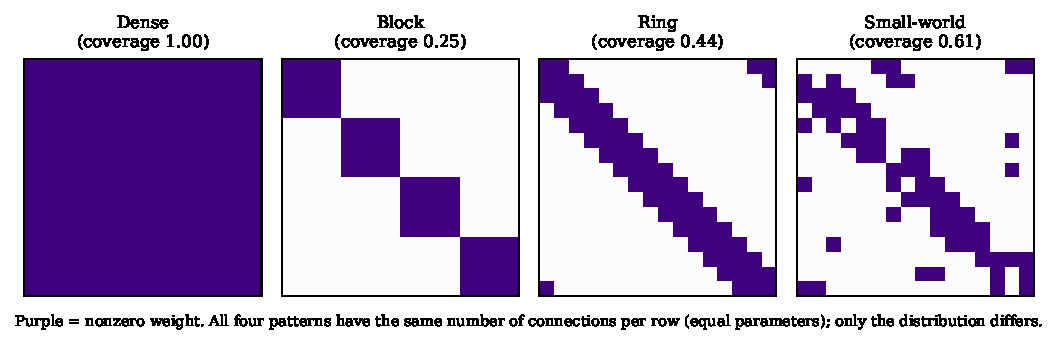
\includegraphics[width=0.92\textwidth]{fig_coverage.pdf}
\caption{The coverage concept. The $16\times16$ weight mask of four connectivity patterns;
purple cells are nonzero weights. All four patterns have the same number of connections per row
(equal parameters); only the distribution, hence coverage, differs.}
\label{fig:coverage}
\end{figure*}

\subsection{Mixing depth}
\label{sec:tau}
Eq.~\eqref{eq:coverage} looks at a single FFN. Information, however, propagates across layers
as well. Writing the reach matrix of layer $\ell$ as $R_\ell = D_\ell U_\ell$, we define the
\emph{cumulative coverage} after $L$ layers,
\begin{equation}
\label{eq:ceff}
\mathcal{C}_{\mathrm{eff}}(L) = \frac{1}{d^2}\sum_{i,j}
  \mathbb{1}\!\left[\left(R_L R_{L-1}\cdots R_1\right)_{ij} > 0\right],
\end{equation}
and from it the \emph{mixing depth}
\begin{equation}
\label{eq:tau}
\tau = \min\{\,L : \mathcal{C}_{\mathrm{eff}}(L) = 1\,\}.
\end{equation}
$\tau$ states how many layers a topology needs before every output can reach every input. Like
$\mathcal{C}$ it is independent of weight values and computable without training, by boolean
matrix products over the masks alone. The two quantities measure different things: the
composition of a block-diagonal mask is again block-diagonal, so for block-diagonal
$\mathcal{C}_{\mathrm{eff}}$ is constant in depth and $\tau$ is undefined ($\tau>L$); the
butterfly, whose stage rotates from layer to layer, completes in
$\lceil \log_2 d \rceil$ layers. And this despite their per-layer coverage being identical
($0.250$).

\emph{How $\tau$ was developed and how it was tested.} We address the risk of fitting a measure
to results already seen (HARKing) explicitly. We formulated $\tau$ on the $M{=}16$ grid, where
we had observed coverage to fail. We then applied it \emph{without modification} to three
independent bodies of data: the other densities ($M \in \{8,32,64\}$), the depth sweep
($L \in \{2,4,8,16\}$), and the distributed variants. Finally, we tested the measure not by
curve-fitting but with two \emph{falsifiable} predictions, both recorded in the experiment
scripts before the corresponding runs were queued:

\begin{enumerate}
\item If the butterfly's stage is frozen across all layers its $\tau$ becomes $>L$; its quality
should then \emph{drop} to the level of block-diagonal, which has the same per-layer coverage
(Section~\ref{sec:fixed}).
\item At $M{=}64$, coverage and $\tau$ give opposite orderings; if measurement follows $\tau$,
butterfly should \emph{overtake} ring, whose coverage is twice as large
(Section~\ref{sec:tau-result}).
\end{enumerate}

Both predictions held. This means $\tau$ was tested as a falsifiable hypothesis rather than
defined post hoc. We report the single case in which the measure fails with the same
discipline.

\subsection{Implementations and controls}
We compute the same math in two ways: \emph{masked} (dense matmul $+$ binary mask; for quality
experiments, treating all variants identically) and \emph{bmm} (real small matrix multiplies;
for speed claims). Because a sparse layer's fan-in is smaller than a dense one's, a single
initialization scale is not neutral; we report results under three initialization regimes
(\texttt{gpt}, \texttt{kaiming}, \texttt{mixed}) separately. To probe the optimization
difficulty of structured layers, we apply, as a control, the self-guided training regime
\cite{wei2024}, which adds a temporary dense branch parallel to the FFN during the first 30\% of
training.

\subsection{Models, data, and statistics}
For the architecture sweep we train GPT-mini ($d{=}512$, 8 layers, $\sim\!25$M) on character-level
\texttt{text8} \cite{mahoney2011} for 6000 steps and measure quality in bits-per-character
(bpc). For scaling we
train a $\sim\!403$M model ($d{=}1024$, 32 layers) on byte-level \texttt{enwik9} using
data-parallel (DDP) over eight H200s with $\sim\!2$B tokens. Distributed measurement is done on
two servers ($2{\times}4$ H200, InfiniBand). All comparisons are reported as mean and standard
deviation over multiple seeds; we measure the significance of a difference by $\sigma = |\Delta|
/ \sqrt{\mathrm{SE}_1^2 + \mathrm{SE}_2^2}$ and treat $\sigma<2$ as noise.

% ============================================================
\section{Results}
% ============================================================
\subsection{Quality and coverage}
Table~\ref{tab:quality} shows the architecture sweep. Sparsity is statistically free up to
density $1/2$ ($\sigma \le 1.2$); at density $1/4$ the dense model wins clearly ($+0.022$ bpc,
$16\sigma$) and the gap grows monotonically as density falls. Within a fixed density, quality
is not determined by the pattern's name: mosaic and block, though seemingly opposite, yield
nearly identical bpc ($0.10\sigma$). We had predicted this equality before seeing the data;
we later realized, however, that mosaic is a row/column permutation of block, and since FFN
hidden units are exchange-symmetric the two variants define the \emph{same model class}. This
equality is therefore not evidence for the coverage hypothesis but a validation of the
experimental pipeline and of the scale of seed noise, and we report it as such. A third
observation is that unstructured random sparsity is better than every structured pattern;
small-world and random are statistically identical at most densities
(Fig.~\ref{fig:density}). This refutes the expectation that ``a regular topology beats random
sparsity'' (for a caveat on its interpretation see Section~\ref{sec:fixed}).

\begin{figure}[!t]
\centering
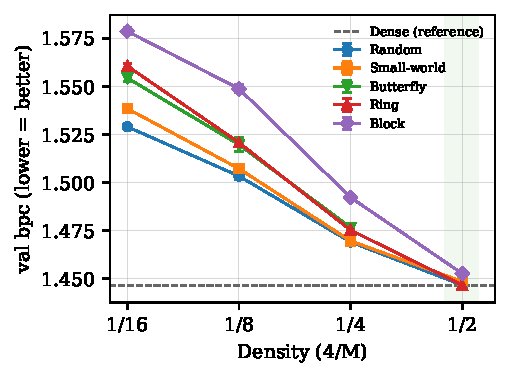
\includegraphics[width=0.95\columnwidth]{fig_density.pdf}
\caption{Density sweep ($L{=}8$, four densities, error bars are standard errors). At density
$1/2$ (green region) all sparse patterns converge to the dense reference (dashed line); as
density falls the patterns diverge, and block --- which never completes its mixing --- is
worst.}
\label{fig:density}
\end{figure}

\begin{figure*}[!t]
\centering
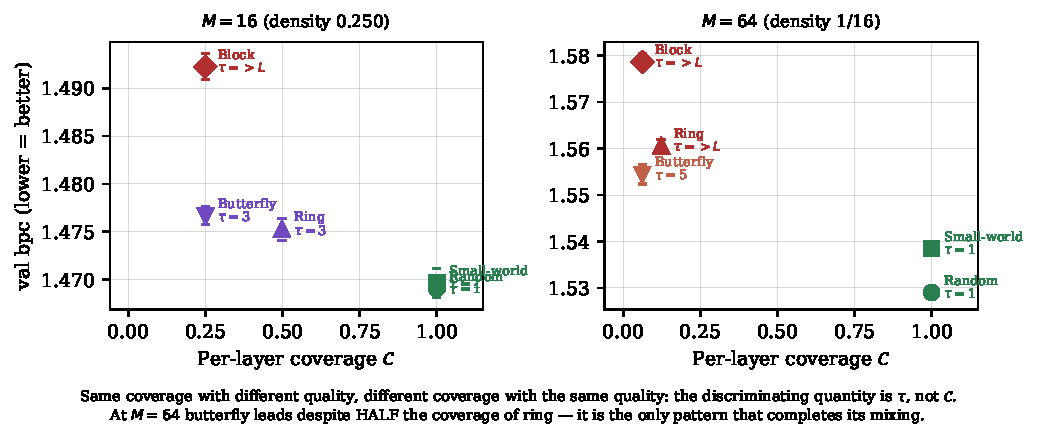
\includegraphics[width=0.92\textwidth]{fig_tau_en.pdf}
\caption{What discriminates quality is mixing depth, not per-layer coverage. Horizontal axis
$\mathcal{C}$, vertical axis val bpc; color encodes $\tau$. Left ($M{=}16$): butterfly and block
share $\mathcal{C}$ yet separate by $9.6\sigma$, while ring and butterfly differ twofold in
$\mathcal{C}$ yet are indistinguishable. Right ($M{=}64$): the two measures disagree in
\emph{order} --- butterfly has half the coverage of ring and still leads, being the only
pattern that completes its mixing.}
\label{fig:tau-fig}
\end{figure*}

\begin{table*}[!t]
\centering
\footnotesize
\caption{Quality: density sweep ($L{=}8$, \texttt{mixed} init, character-level \texttt{text8},
bpc). $\sigma$: ratio of the gap to combined standard error vs.\ dense; $\sigma<2$ is noise.
$n$: seeds.}
\label{tab:quality}
\begin{tabular}{@{}llccccc@{}}
\toprule
Pattern & $M$ & Density & Coverage & val bpc & Gap vs.\ dense & $\sigma$ \\
\midrule
Dense          & 8  & 0.500 & 1.000 & 1.4466 & ---       & ---  \\
Ring           & 8  & 0.500 & 0.998 & 1.4467 & $+0.0001$ & 0.1  \\
Random         & 8  & 0.500 & 1.000 & 1.4467 & $+0.0001$ & 0.0  \\
Small-world    & 8  & 0.500 & 1.000 & 1.4485 & $+0.0019$ & 1.2  \\
Block          & 8  & 0.500 & 0.500 & 1.4527 & $+0.0061$ & 3.5  \\
Mosaic         & 8  & 0.500 & 0.500 & 1.4541 & $+0.0075$ & 3.9  \\
\midrule
Random         & 16 & 0.250 & 1.000 & 1.4691 & $+0.0225$ & 16.4 \\
Small-world    & 16 & 0.250 & 1.000 & 1.4696 & $+0.0230$ & 13.3 \\
Ring           & 16 & 0.250 & 0.498 & 1.4752 & $+0.0286$ & 19.4 \\
Butterfly      & 16 & 0.250 & 0.250 & 1.4766 & $+0.0300$ & 14.2 \\
Block          & 16 & 0.250 & 0.250 & 1.4923 & $+0.0457$ & 28.4 \\
Mosaic         & 16 & 0.250 & 0.250 & 1.4925 & $+0.0459$ & 18.4 \\
\midrule
Random         & 32 & 0.125 & 1.000 & 1.5034 & $+0.0568$ & 28.2 \\
Small-world    & 32 & 0.125 & 1.000 & 1.5072 & $+0.0606$ & 40.4 \\
Butterfly      & 32 & 0.125 & 0.125 & 1.5197 & $+0.0731$ & 20.3 \\
Ring           & 32 & 0.125 & 0.248 & 1.5208 & $+0.0742$ & 58.9 \\
Block          & 32 & 0.125 & 0.125 & 1.5488 & $+0.1022$ & 44.2 \\
\midrule
Random         & 64 & 0.062 & 1.000 & 1.5290 & $+0.0824$ & 61.3 \\
Small-world    & 64 & 0.062 & 1.000 & 1.5385 & $+0.0919$ & 88.7 \\
Butterfly      & 64 & 0.062 & 0.062 & 1.5544 & $+0.1078$ & 48.1 \\
Ring           & 64 & 0.062 & 0.123 & 1.5606 & $+0.1140$ & 72.5 \\
Block          & 64 & 0.062 & 0.062 & 1.5787 & $+0.1321$ & 68.2 \\
\bottomrule
\end{tabular}
\end{table*}

\subsection{Where coverage fails: mixing depth}
\label{sec:tau-result}
Per-layer coverage $\mathcal{C}$ gives the coarse ordering but misleads in both directions. At
$M{=}16$ butterfly and block have the \emph{same} coverage ($0.250$) yet differ by $0.0156$ bpc,
i.e.\ $9.6\sigma$; conversely ring and butterfly differ in coverage by a \emph{factor of two}
($0.498$ vs.\ $0.250$) yet the measured gap is $0.0014$ bpc, i.e.\ $0.95\sigma$ --- noise.
Coverage rules wrongly in both cases.

The mixing depth $\tau$ of Eq.~\eqref{eq:tau} corrects both (Table~\ref{tab:tau}). What decides
quality is whether mixing \emph{completes}: the gap between any pattern with $\tau \le L$ and
any pattern with $\tau > L$ is significant at every density (weakest separation $2.03\sigma$ at
$M{=}8$, $6.33\sigma$ at $M{=}16$; Fig.~\ref{fig:tau-fig}). The mechanism is structural: the composition of block and
mosaic remains block-diagonal, so $\mathcal{C}_{\mathrm{eff}}$ stays pinned at $0.25$ regardless
of depth, whereas the butterfly reaches $1.0$ in three layers. Among completing patterns quality
degrades with $\tau$, and patterns with equal $\tau$ are indistinguishable ($\sigma \le 0.95$);
the resolution of this graded ordering, however, depends on sparsity: at $M{=}16$ the
$\tau{=}1$ and $\tau{=}3$ tiers separate ($2.96\sigma$), while at $M{=}8$ the $\tau{=}1$ versus
$\tau{=}2$ difference falls below noise ($0.02\sigma$). $\tau$ is thus an ordinal measure, not
a metric.

\emph{Independent replication.} The ``same coverage, different quality'' counterexample is not
specific to one density: at $M{=}32$ butterfly and block again share a coverage of $0.125$ and
separate by $7.1\sigma$; at $M{=}64$ they share $0.062$ and separate by $9.0\sigma$. At all
three densities the discriminating quantity is $\tau$.

\emph{A case where the two measures rule oppositely.} $M{=}64$ provides a cell in which
coverage and $\tau$ disagree not in magnitude but in \emph{order}. There the ring's per-layer
coverage ($0.123$) is twice the butterfly's ($0.062$), so coverage ranks ring ahead. But the
ring cannot finish mixing in eight layers ($\mathcal{C}_{\mathrm{eff}}{=}0.971$, $\tau>L$) while
the butterfly does ($\tau{=}5$); $\tau$ ranks butterfly ahead. Measurement confirms $\tau$:
butterfly $1.5544$ versus ring $1.5606$ ($2.53\sigma$). The pattern with half the coverage wins
because it can complete its mixing. This prediction was recorded before the runs.

\emph{The one failure of $\tau$.} Across four densities, of 41 pairwise comparisons 35 are
correct, nine are statistically indistinguishable, and \emph{one} is a violation. The ordering
is never inverted; the single defect is a failure to discriminate: at $M{=}64$ random and
small-world both have $\tau{=}1$ yet separate by $8.2\sigma$. This is an expected limit ---
$\tau$ is a binary reachability measure and does not see the \emph{distribution} of that reach;
when only 32 connections per row remain, ``reaches every input'' is too coarse a statement to
determine quality.

\begin{table}[!t]
\centering
\footnotesize
\caption{Mixing depth $\tau$ explains what per-layer coverage cannot ($M{=}16$, $L{=}8$).
Butterfly and block share $\mathcal{C}$ but differ in $\tau$; ring and butterfly differ in
$\mathcal{C}$ but share $\tau$. Measurement follows $\tau$: patterns with equal $\tau$ are
indistinguishable, those with different $\tau$ are significant.}
\label{tab:tau}
\begin{tabular}{@{}lccccc@{}}
\toprule
Pattern & Across layers & $\mathcal{C}$ & $\tau$ & val bpc & $n$ \\
\midrule
Random      & varying & 1.000 & 1     & $1.4691 \pm 0.0023$ & 9 \\
Small-world & varying & 1.000 & 1     & $1.4696 \pm 0.0036$ & 6 \\
\midrule
Ring        & fixed   & 0.498 & 3     & $1.4752 \pm 0.0029$ & 6 \\
Butterfly   & varying & 0.250 & 3     & $1.4766 \pm 0.0023$ & 6 \\
\midrule
Block       & fixed   & 0.250 & $>L$  & $1.4923 \pm 0.0023$ & 3 \\
Mosaic      & fixed   & 0.250 & $>L$  & $1.4925 \pm 0.0040$ & 3 \\
\bottomrule
\end{tabular}
\end{table}

\subsection{Depth: the interaction of $\tau$ and $L$}
Table~\ref{tab:depth} shows how the gap between ring and random changes with depth. It does not
grow monotonically; it traces $2.8\sigma \to 0.3\sigma \to 4.3\sigma \to 23.3\sigma$
(Fig.~\ref{fig:depth}). This non-monotone trajectory is explained by comparing $\tau$ with $L$,
which yields three regimes.

In the $L<\tau$ regime ($L{=}2$) the ring cannot complete its mixing and pays a penalty. In the
$L\approx\tau$ regime ($L{=}4$, where $\tau{=}3$ for ring) mixing finishes exactly, and the gap
\emph{closes} ($0.3\sigma$; the sign even reverses, i.e.\ the difference falls entirely into
noise); this is the one point at which depth genuinely rescues weak mixing. In the $L>\tau$
regime ($L{=}8,16$) the gap widens again, because the binding constraint is no longer coverage
but \emph{saturation}: past $\tau$ a fixed pattern adds no new connections, whereas a pattern
that varies across layers applies fresh mixing at every layer. The depth finding is thus not a
single effect but the intersection of two mechanisms (the $\tau$ threshold and saturation). The
second mechanism is what ShuffleSparse \cite{shufflesparse2025} predicts, and we confirm it with
independent measurement.

$\tau$ does not order all of these rows. At $L{=}2$ every sparse variant beats the dense model
by a wide margin ($\sim\!0.07$ bpc): in a shallow network the hidden layer widened by the
equal-parameter protocol dominates topology differences. In that row the spread across patterns
falls to $0.009$ bpc and butterfly --- the variant with the lowest cumulative coverage ---
comes out nominally best. Mixing depth is therefore not explanatory in the shallow regime;
width dominates.

\begin{figure}[!t]
\centering
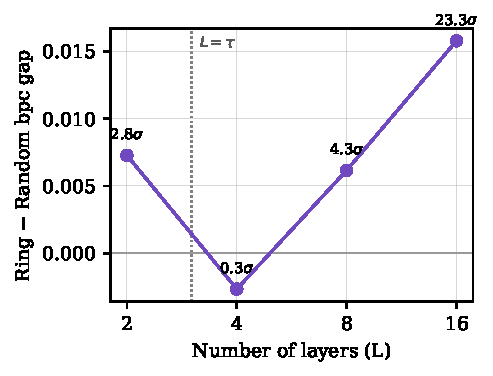
\includegraphics[width=0.95\columnwidth]{fig_depth.pdf}
\caption{The ring$-$random bpc gap as a function of depth ($M{=}16$). The gap reaches
$20.3\sigma$ at $L{=}16$; a fixed pattern (ring) cannot exploit depth, so the gap widens. Labels
show statistical significance ($\sigma$).}
\label{fig:depth}
\end{figure}

\begin{table}[!t]
\centering
\footnotesize
\caption{Depth: the ring$-$random gap does not grow monotonically but closes at the $\tau$
threshold ($M{=}16$, \texttt{mixed}). For ring $\tau{=}3$; the gap vanishes only when
$L{\approx}\tau$ and reopens through saturation when $L>\tau$.}
\label{tab:depth}
\begin{tabular}{@{}lcccccc@{}}
\toprule
$L$ & Regime & Dense & Rand. & Ring & Butterfly & R$-$R ($\sigma$) \\
\midrule
2  & $L<\tau$       & 1.6338 & 1.5664 & 1.5736 & 1.5650 & $+0.0073$ (2.8) \\
4  & $L\approx\tau$ & 1.5285 & 1.5454 & 1.5428 & 1.5420 & $-0.0027$ (0.3) \\
8  & $L>\tau$       & 1.4466 & 1.4691 & 1.4752 & 1.4766 & $+0.0062$ (4.3) \\
16 & $L>\tau$       & 1.4024 & 1.4364 & 1.4521 & 1.4463 & $+0.0158$ (23.3) \\
\bottomrule
\end{tabular}
\end{table}

\subsection{The fixed-mask control: disentangling two findings}
\label{sec:fixed}
In our initial setup the two findings above --- ``unstructured random is best'' and
``depth-varying patterns are advantaged'' --- were not separable. To reduce variance our
implementation gives each layer a different mask seed; as a side effect, patterns that consume
the seed (random, small-world) are \emph{redrawn} from layer to layer, and the butterfly already
varies through its stage. The random control group was therefore itself a depth-varying pattern.

To separate them we ran a control that fixes the topology across all layers while still varying
it across seeds (so variance reduction is preserved and only the depth axis is closed).
Eq.~\eqref{eq:tau} yields two \emph{falsifiable} predictions for this control, and we recorded
them before the runs: (i) fixed random also has $\tau{=}1$, so its quality should
\emph{not change}; (ii) the butterfly with a frozen stage has $\tau>L$, so it should
\emph{drop} to the level of block. In addition the flag is inert for ring by construction,
which we use as a null control. Results are in Table~\ref{tab:fixed}.

The null control passed: for ring the fixed-versus-varying difference is $0.49\sigma$; matched
by seed, the mean absolute difference is $0.0012$ bpc, one third of the across-seed standard
deviation ($0.0033$), and its sign varies from seed to seed --- this is run-to-run
nondeterminism from TF32 and atomic reductions, not a systematic effect.

The first prediction held: fixed random was indistinguishable from its varying counterpart at
all three depths ($0.88\sigma$, $0.48\sigma$, $1.26\sigma$). The finding that ``unstructured
random is best'' is thus a coverage effect and not an artifact of redrawing across layers; the
two findings are independent.

The second prediction held quantitatively and is the strongest evidence for $\tau$. With its
stage frozen the butterfly falls from $1.4766$ to $1.4927$ at $L{=}8$ ($5.4\sigma$) --- and that
value lies $0.14\sigma$ from block's $1.4923$, which has the same coverage. $\tau$ thus
predicted not merely a direction but a \emph{point}, and hit it: what separates butterfly from
block is neither its connection count nor its per-layer coverage, but only the rotation of its
stage across layers. The effect grows with depth ($+0.0064 \to +0.0161 \to +0.0373$), as the
saturation mechanism expects: a fixed pattern wastes every layer beyond $\tau$. At $L{=}4$ the
difference is in the right direction but not significant ($1.08\sigma$); at that depth the total
spread across patterns is itself only $\sim\!0.02$ bpc.

\begin{table}[!t]
\centering
\footnotesize
\caption{The fixed-mask control ($M{=}16$). Topology is fixed across all layers and still varies
across seeds. Predictions were recorded before the runs.}
\label{tab:fixed}
\begin{tabular}{@{}llccc@{}}
\toprule
Pattern & $L$ & Varying & Fixed & $\Delta$ ($\sigma$) \\
\midrule
\multicolumn{5}{@{}l}{\emph{Null control} --- prediction: inert} \\
Ring      & 8  & 1.4752 & 1.4764 & $+0.0011$ (0.5) \\
\midrule
\multicolumn{5}{@{}l}{\emph{Main control} --- prediction: no change ($\tau{=}1 \to 1$)} \\
Random    & 4  & 1.5454 & 1.5508 & $+0.0054$ (0.9) \\
Random    & 8  & 1.4691 & 1.4698 & $+0.0008$ (0.5) \\
Random    & 16 & 1.4364 & 1.4346 & $-0.0017$ (1.3) \\
\midrule
\multicolumn{5}{@{}l}{\emph{Sharp test} --- prediction: drop to block ($\tau{=}3 \to {>}L$)} \\
Butterfly & 4  & 1.5420 & 1.5484 & $+0.0064$ (1.1) \\
Butterfly & 8  & 1.4766 & \textbf{1.4927} & $+0.0161$ (5.4) \\
Butterfly & 16 & 1.4463 & 1.4836 & $+0.0373$ (28.9) \\
\midrule
\multicolumn{5}{@{}l}{Block ($L{=}8$, same $\mathcal{C}{=}0.250$): $1.4923$ ---
$0.14\sigma$ from fixed butterfly} \\
\bottomrule
\end{tabular}
\end{table}

\subsection{Control experiments}
\emph{Initialization scale.} We observed that sparse layers inject a differently scaled signal
into GELU (output std $1.41$ vs.\ $0.45$). We repeated all main findings under three
initialization regimes; the coverage ordering held in all three, so the results are independent
of the initialization choice.

\emph{Self-guided training.} The gain shows a phase transition (Table~\ref{tab:guide}): there is
no significant effect at $L\le 8$, but at $L{=}16$ a significant improvement appears in all three
patterns. Un-guided deep models did not stall; the gain is not a ``rescue'' but a $\sim\!1\%$
improvement. Critically, under guidance the apparent superiority of butterfly over ring vanishes
($12.0\sigma \to 1.5\sigma$), showing that the naive reading ``depth-varying patterns give better
\emph{quality}'' is largely an optimization artifact. The correct statement is: butterfly gives
the \emph{same} quality as ring with half the communication.

\begin{table}[!t]
\centering
\footnotesize
\caption{Effect of self-guided training by depth ($M{=}16$). Phase transition: no effect at
$L\le8$, significant at $L{=}16$.}
\label{tab:guide}
\begin{tabular}{@{}llccc@{}}
\toprule
$L$ & Pattern & Un-guided & Guided & Gain ($\sigma$) \\
\midrule
8  & Butterfly & 1.4765 & 1.4727 & $+0.0038$ (1.8) \\
8  & Random    & 1.4682 & 1.4696 & $-0.0014$ (0.9) \\
8  & Ring      & 1.4752 & 1.4724 & $+0.0028$ (1.5) \\
16 & Butterfly & 1.4457 & 1.4339 & $+0.0118$ (13.5) \\
16 & Random    & 1.4373 & 1.4273 & $+0.0099$ (4.9)  \\
16 & Ring      & 1.4521 & 1.4363 & $+0.0158$ (10.6) \\
\bottomrule
\end{tabular}
\end{table}

\subsection{Distributed communication}
Table~\ref{tab:dist} shows values measured on eight H200s at equal per-rank parameters. Butterfly
sharding reduces peers from $7$ to $1$ and FFN communication volume by $\sim\!7\times$, and is
faster than ring and dense TP in the forward pass. \emph{Important caveat:} this $7\times$ is for
the FFN only; because the attention layer also requires an all-reduce in both strategies, the
end-to-end communication reduction is limited to $\sim\!2\times$. In a separate experiment we
trained an attention-free FFN stack end-to-end on eight H200s; at equal per-rank parameters the
wide-sparse variants (ring $2.02$, butterfly $2.04$ bpc) clearly beat narrow-dense tensor
parallelism ($2.73$), confirming that distributed sharding is genuinely trainable.

\begin{table}[!t]
\centering
\footnotesize
\caption{Distributed communication ($8{\times}$H200, $d{=}8192$, equal per-rank parameters).}
\label{tab:dist}
\begin{tabular}{@{}lccc@{}}
\toprule
Sharding & Comm. (MB/step) & Peers & Forward (ms) \\
\midrule
Dense tensor-parallel & 469.8 & 7 & 4.25 \\
Ring                  & 134.2 & 2 & 2.83 \\
Butterfly             & 67.1  & 1 & 2.51 \\
Block                 & 0.0   & 0 & 1.90 \\
\bottomrule
\end{tabular}
\end{table}

\subsection{Implementation and scaling}
We verified that the bmm implementation of butterfly gives the same quality as the masked one
(gap $\le 0.0007$ bpc), but bmm is $\sim\!1.9\times$ \emph{slower} at this scale: the gather and
concatenate steps required by the XOR pairing are memory-bound. This is implementation-specific;
Monarch \cite{dao2022} achieves $2\times$ speedup on the same structure with a fused kernel. At
scale ($\sim\!403$M, Table~\ref{tab:scale}) the dense model's $0.91$ bpc is in the range of strong
baselines. The ordering of the means matches the small scale (dense $\le$ random $\le$
butterfly), but applying our own $\sigma\!\ge\!2$ criterion to this table requires reporting it
as it stands: at this scale the dense-to-random difference is \emph{not significant}
($+0.0097$ bpc, $1.34\sigma$, $n{=}2$), and dense-to-butterfly is borderline ($1.95\sigma$); the
dense model's spread across two seeds ($\pm0.0101$) exceeds the difference itself. The only
comparison that remains significant is random versus butterfly ($+0.0043$ bpc, $5.36\sigma$),
and that gap halves relative to the small scale ($12.5\sigma \to 5.4\sigma$) without closing.
What this experiment supports is therefore not ``the quality cost of sparsity persists at
403M'' but ``that cost has sunk into measurement noise at this budget''; two seeds are
insufficient for a stronger claim.

\begin{table}[!t]
\centering
\footnotesize
\caption{Scaling: $\sim\!403$M ($d{=}1024$, $L{=}32$, byte-level \texttt{enwik9}, 2 seeds).
Memory/speed refer to the masked implementation.}
\label{tab:scale}
\begin{tabular}{@{}lcccc@{}}
\toprule
Pattern & val bpc & $\pm$ & Memory (GB) & k tok/s \\
\midrule
Dense     & 0.9096 & 0.0101 & 38 & 771 \\
Random    & 0.9193 & 0.0011 & 99 & 329 \\
Butterfly & 0.9236 & 0.0003 & 99 & 337 \\
\bottomrule
\end{tabular}
\end{table}

% ============================================================
\section{Information-Theoretic Bound}
\label{sec:bound}
% ============================================================
In an FFN layer split into $P$ shards, if a shard communicates with $k$ other shards, the output
units it can compute in that layer can depend on at most a fraction $(k{+}1)/P$ of the inputs.
Hence the per-layer coverage is bounded by
\begin{equation}
\mathcal{C}_{\text{layer}} \le \frac{k+1}{P} .
\end{equation}
Full coverage ($\mathcal{C}_{\text{layer}}{=}1$) is possible only with $k{=}P{-}1$ (all-to-all).
An impossibility follows: full per-layer coverage and single-peer ($k{=}1$) communication cannot
coexist in one layer. Full mixing with a single peer is achievable only over depth: butterfly
reaches full mixing in $\log_2(P)$ layers by pairing with a different partner ($r\oplus 2^\ell$)
at each layer, while fixed-neighbor ring requires $P/2$ layers. Recovering coverage over depth
carries a small but persistent quality cost (our measured butterfly--random gap thins with scale
but does not close). This is not an engineering shortcoming but a law that bounds the design space.

% ============================================================
\section{Decision Model}
% ============================================================
Butterfly sharding is rational only when three conditions hold simultaneously: (i) the model is
too large to fit in one data center; (ii) the inter-center link is too narrow for dense TP; but
(iii) fast enough for butterfly. Using the measured communication values, the model shows that
this corridor opens in practice for links above $\sim\!400$ Gbps (same-city / dedicated fiber),
while on consumer internet even butterfly is insufficient (Table~\ref{tab:decision}). In the big
picture, inter-center layer-by-layer sharding is almost always a bad idea; butterfly's real home
is large intra-cluster deployments where many nodes are connected by a fast fabric.

\begin{table}[!t]
\centering
\footnotesize
\caption{Decision-model examples. Butterfly is rational only in a narrow corridor.}
\label{tab:decision}
\begin{tabular}{@{}p{3.0cm}p{1.5cm}p{2.4cm}@{}}
\toprule
Scenario & Regime & Decision \\
\midrule
7B, fits one center       & ---           & Do not split; data-parallel \\
500B, 400 Gbps dedicated  & corridor      & \textbf{Use butterfly} \\
500B, 100 Gbps            & link-bound    & Even butterfly insufficient \\
500B, consumer internet   & link-bound    & Do not attempt model-parallel \\
\bottomrule
\end{tabular}
\end{table}

% ============================================================
\section{Limitations}
\label{sec:limits}
% ============================================================
(1) Only the FFN was sharded; because attention also needs an all-reduce, the end-to-end gain is
limited to $\sim\!2\times$. (2) The bmm implementation is naive and slow at this scale; a fused
kernel could reverse this. (3) The memory cost in the quality experiments stems from our choice
to widen the hidden layer for a fair comparison; it does not arise in a sharded implementation.
(4) End-to-end training over a real wide-area network was not performed; the decision model
rests on bandwidth alone and includes neither latency nor loss. (5) The mechanism behind
the optimization difficulty was not measured, only its outcome. (6) Per-layer coverage alone is
insufficient (a $9.6\sigma$ difference at identical coverage); the mixing depth $\tau$ resolves
these counterexamples but is an ordinal measure: small $\tau$ differences fall below noise at
low sparsity, and in a shallow network ($L{=}2$) it is not explanatory at all because the width
effect dominates.

(7) $\tau$ held both of its predictions in the fixed-mask control (Section~\ref{sec:fixed}), but
that control was confined to $M{=}16$ and $L\in\{4,8,16\}$; it was not repeated at other
densities or for the other seed-consuming patterns such as small-world. Moreover $\tau$ is a
binary reachability measure and does not see the distribution of that reach; in the sparsest
regime ($M{=}64$) we measured a case in which it cannot discriminate two patterns with the same
$\tau$ ($8.2\sigma$).

(8) Experiments are on character-level \texttt{text8} and byte-level \texttt{enwik9}; since the
FFN's mixing burden may differ for models using a subword (BPE) vocabulary, transfer of these
findings to that regime is unverified.

% ============================================================
\section{Conclusion}
% ============================================================
This work proposes no method; it maps a trade-off. We showed that abandoning the dense FFN matrix
assumption yields no quality gain on a single accelerator; that it is free up to
density $1/2$ and costly beyond; and that unstructured random sparsity is better than every
structured pattern. On speed our claim is narrower: \emph{our} masked and bmm implementations
produced no speedup, which we attribute to memory-bound gather/concatenate steps; given that a
fused kernel may reverse this \cite{dao2022}, we draw no general conclusion of the form
``structured sparsity does not accelerate.'' We measured that quality is determined not by
per-layer coverage but by mixing depth, and that the effect of depth changes direction at the
$\tau$ threshold. We established that the gain appears only in distributed communication ---
butterfly gives the same quality as ring with half the communication and a single peer --- but
that it is subject to an information-theoretic bound and a small, persistent quality cost. We
showed that the initial goal of ``uniting scattered resources over the internet'' is not solved
by changing the weight structure. The contribution is a controlled map of where the fundamental
trade-off between communication and quality lies: the result is not a recipe but a compass.

\emph{Reproducibility.} All experiments (326 runs) were repeated with multiple seeds; the code,
SLURM scripts, and raw result files are kept openly.

% ============================================================
\section*{Acknowledgment}
% ============================================================
The numerical calculations reported in this paper were fully performed at TUBITAK ULAKBIM, High
Performance and Grid Computing Center (TRUBA resources).

% ============================================================
\begin{thebibliography}{1}
\bibitem{wei2024}
X. Wei, S. Moalla, R. Pascanu, and C. Gülçehre, ``Building on efficient foundations: Effectively
training LLMs with structured feedforward layers,'' in \emph{Proc. Adv. Neural Inf. Process.
Syst. (NeurIPS)}, 2024.

\bibitem{dao2022}
T. Dao \emph{et al.}, ``Monarch: Expressive structured matrices for efficient and accurate
training,'' in \emph{Proc. Int. Conf. Mach. Learn. (ICML)}, 2022. [Online]. Available:
arXiv:2204.00595.

\bibitem{vaswani2017}
A. Vaswani \emph{et al.}, ``Attention is all you need,'' in \emph{Proc. Adv. Neural Inf.
Process. Syst. (NeurIPS)}, 2017, pp.~5998--6008.

\bibitem{kaplan2020}
J. Kaplan \emph{et al.}, ``Scaling laws for neural language models,'' 2020. [Online].
Available: arXiv:2001.08361.

\bibitem{chinchilla2022}
J. Hoffmann \emph{et al.}, ``Training compute-optimal large language models,'' in
\emph{Proc. Adv. Neural Inf. Process. Syst. (NeurIPS)}, 2022.

\bibitem{megatron2019}
M. Shoeybi, M. Patwary, R. Puri, P. LeGresley, J. Casper, and B. Catanzaro, ``Megatron-LM:
Training multi-billion parameter language models using model parallelism,'' 2019. [Online].
Available: arXiv:1909.08053.

\bibitem{narayanan2021}
D. Narayanan \emph{et al.}, ``Efficient large-scale language model training on GPU clusters
using Megatron-LM,'' in \emph{Proc. Int. Conf. High Perform. Comput., Netw., Storage Anal.
(SC)}, 2021.

\bibitem{zero2020}
S. Rajbhandari, J. Rasley, O. Ruwase, and Y. He, ``ZeRO: Memory optimizations toward training
trillion parameter models,'' in \emph{Proc. Int. Conf. High Perform. Comput., Netw., Storage
Anal. (SC)}, 2020.

\bibitem{fsdp2023}
Y. Zhao \emph{et al.}, ``PyTorch FSDP: Experiences on scaling fully sharded data parallel,''
\emph{Proc. VLDB Endow.}, vol.~16, no.~12, pp.~3848--3860, 2023.

\bibitem{gpipe2019}
Y. Huang \emph{et al.}, ``GPipe: Efficient training of giant neural networks using pipeline
parallelism,'' in \emph{Proc. Adv. Neural Inf. Process. Syst. (NeurIPS)}, 2019.

\bibitem{korthikanti2023}
V. Korthikanti \emph{et al.}, ``Reducing activation recomputation in large transformer
models,'' in \emph{Proc. Mach. Learn. Syst. (MLSys)}, 2023.

\bibitem{ringattn2023}
H. Liu, M. Zaharia, and P. Abbeel, ``Ring attention with blockwise transformers for
near-infinite context,'' 2023. [Online]. Available: arXiv:2310.01889.

\bibitem{han2015}
S. Han, J. Pool, J. Tran, and W. Dally, ``Learning both weights and connections for efficient
neural networks,'' in \emph{Proc. Adv. Neural Inf. Process. Syst. (NeurIPS)}, 2015.

\bibitem{frankle2019}
J. Frankle and M. Carbin, ``The lottery ticket hypothesis: Finding sparse, trainable neural
networks,'' in \emph{Proc. Int. Conf. Learn. Represent. (ICLR)}, 2019.

\bibitem{rigl2020}
U. Evci, T. Gale, J. Menick, P. S. Castro, and E. Elsen, ``Rigging the lottery: Making all
tickets winners,'' in \emph{Proc. Int. Conf. Mach. Learn. (ICML)}, 2020.

\bibitem{sparsegpt2023}
E. Frantar and D. Alistarh, ``SparseGPT: Massive language models can be accurately pruned in
one-shot,'' in \emph{Proc. Int. Conf. Mach. Learn. (ICML)}, 2023.

\bibitem{nm2021}
A. Mishra \emph{et al.}, ``Accelerating sparse deep neural networks,'' 2021. [Online].
Available: arXiv:2104.08378.

\bibitem{expander2018}
A. Prabhu, G. Varma, and A. Namboodiri, ``Deep expander networks: Efficient deep networks from
graph theory,'' in \emph{Proc. Eur. Conf. Comput. Vis. (ECCV)}, 2018.

\bibitem{dao2019}
T. Dao, A. Gu, M. Eichhorn, A. Rudra, and C. Ré, ``Learning fast algorithms for linear
transforms using butterfly factorizations,'' in \emph{Proc. Int. Conf. Mach. Learn. (ICML)},
2019.

\bibitem{pixelbutterfly2022}
B. Chen, T. Dao, K. Liang, J. Yang, Z. Song, A. Rudra, and C. Ré, ``Pixelated butterfly:
Simple and efficient sparse training for neural network models,'' in \emph{Proc. Int. Conf.
Learn. Represent. (ICLR)}, 2022.

\bibitem{shazeer2017}
N. Shazeer \emph{et al.}, ``Outrageously large neural networks: The sparsely-gated
mixture-of-experts layer,'' in \emph{Proc. Int. Conf. Learn. Represent. (ICLR)}, 2017.

\bibitem{gshard2021}
D. Lepikhin \emph{et al.}, ``GShard: Scaling giant models with conditional computation and
automatic sharding,'' in \emph{Proc. Int. Conf. Learn. Represent. (ICLR)}, 2021.

\bibitem{stich2019}
S. U. Stich, ``Local SGD converges fast and communicates little,'' in \emph{Proc. Int. Conf.
Learn. Represent. (ICLR)}, 2019.

\bibitem{swarm2023}
M. Ryabinin, T. Dettmers, M. Diskin, and A. Borzunov, ``SWARM parallelism: Training large
models can be surprisingly communication-efficient,'' in \emph{Proc. Int. Conf. Mach. Learn.
(ICML)}, 2023.

\bibitem{petals2023}
A. Borzunov \emph{et al.}, ``Petals: Collaborative inference and fine-tuning of large models,''
in \emph{Proc. Assoc. Comput. Linguistics (ACL), System Demonstrations}, 2023.

\bibitem{mahoney2011}
M. Mahoney, ``Large text compression benchmark,'' 2011. [Online]. Available:
http://mattmahoney.net/dc/text.html.

\bibitem{switch2022}
W. Fedus, B. Zoph, and N. Shazeer, ``Switch Transformer: Scaling to trillion parameter models
with simple and efficient sparsity,'' \emph{J. Mach. Learn. Res.}, vol.~23, no.~120,
pp.~1--39, 2022.

\bibitem{diloco2023}
A. Douillard \emph{et al.}, ``DiLoCo: Distributed low-communication training of language
models,'' 2023. [Online]. Available: arXiv:2311.08105.

\bibitem{shufflesparse2025}
A. Tyagi \emph{et al.}, ``ShuffleSparse: Learned shuffles for structured sparse networks,'' 2025.
[Online]. Available: arXiv:2510.14812.

\bibitem{bdlora2025}
``Block-diagonal LoRA for eliminating communication overhead in tensor parallel LoRA serving,''
2025. [Online]. Available: arXiv:2510.23346.

\bibitem{detransformer2024}
``Communication-efficient model parallelism for distributed in-situ transformer inference,'' in
\emph{Proc. Design, Automation Test Eur. Conf. (DATE)}, 2024.

\bibitem{flashcomm2024}
``Flash communication: Reducing tensor parallelization bottleneck for fast LLM inference,'' 2024.
[Online]. Available: arXiv:2412.04964.
\end{thebibliography}

\end{document}
